\section{Experimental Measurements and Results}
\label{sec:exp_results}

To evaluate the performance and scalability of the PAKE protocols, we conducted a series of experiments on the server-side implementation. The goal was to measure the impact of the different PAKE protocols on the system's resource utilization, including CPU usage and storage requirements, to understand the practical implications of adopting these protocols in real-world applications.

Our benchmark simulated a high-pressure user registration and login scenario, with 10 concurrent user threads performing 1,000 rounds of registration and login. The results showed a significant difference in the CPU usage patterns between the PAKE protocols and the basic password-over-TLS authentication.

\begin{figure}[ht]
  \centering
  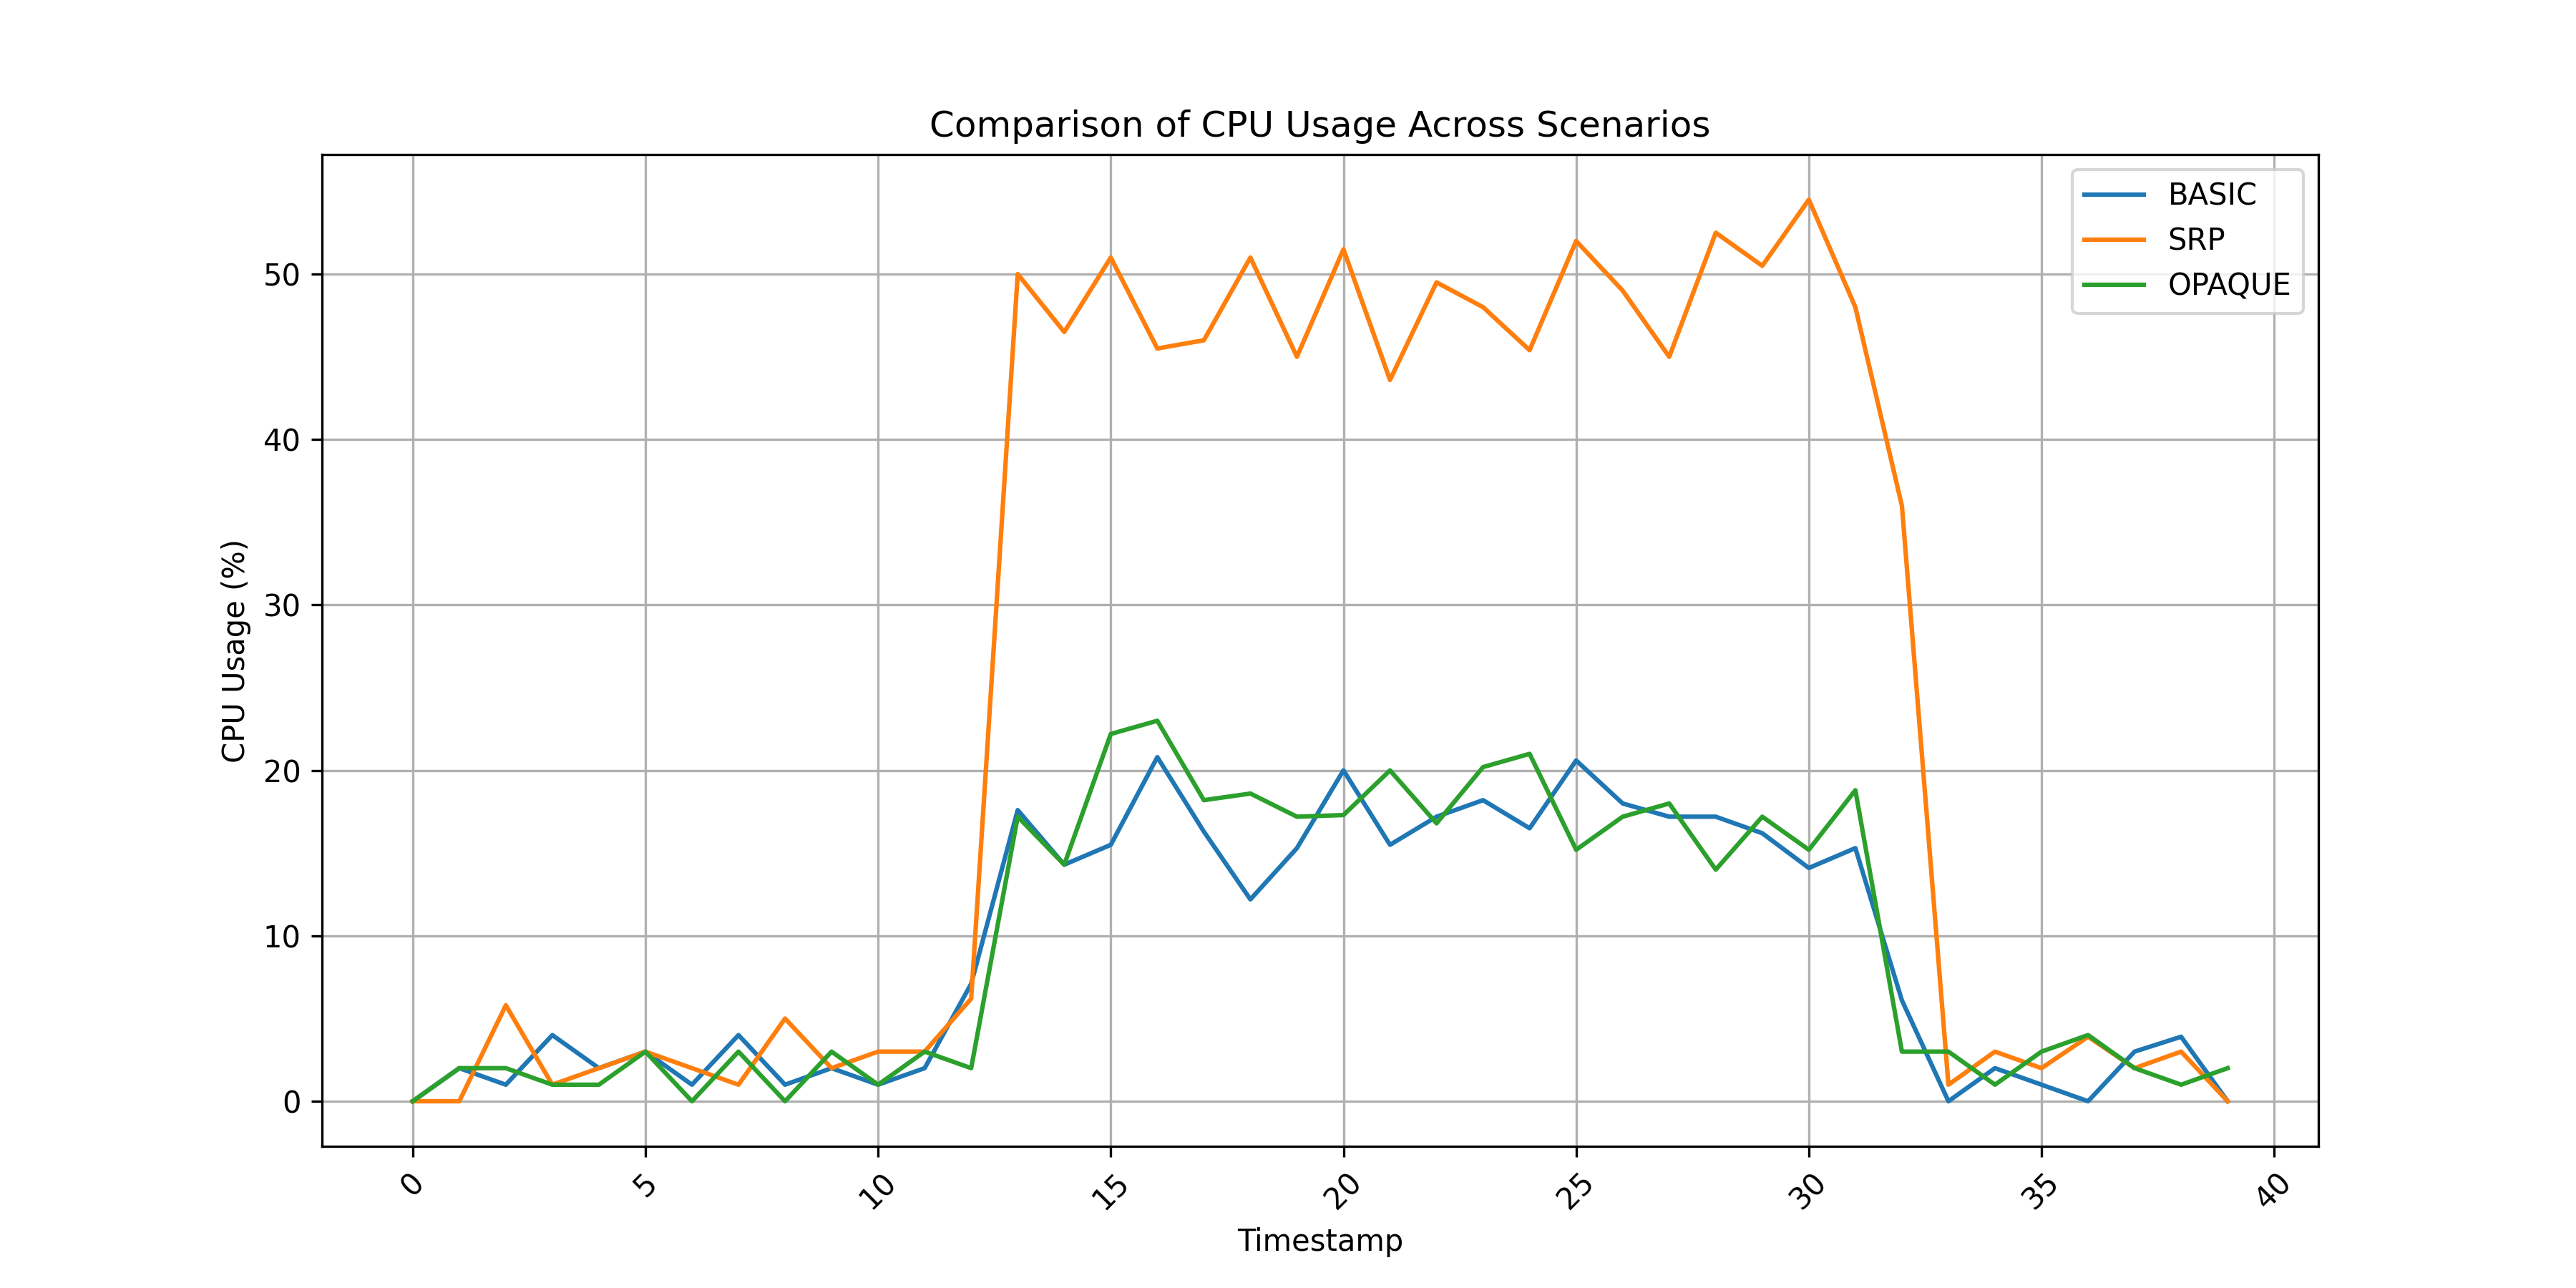
\includegraphics[width=0.4\textwidth]{./images/cpu_usage_comparison.png}
  \caption{Comparison of server-side CPU usage}
  \label{fig:cpu_usage}
\end{figure}

\subsection{Server-side CPU Usage}

One of the key performance metrics we examined was the server-side CPU utilization over time. The PAKE protocols, by nature, involve more complex cryptographic operations compared to a basic password-over-TLS authentication, which could potentially lead to higher CPU consumption.

As shown in Figure \ref{fig:cpu_usage}, the Password Over TLS protocol exhibited a relatively stable and low CPU usage throughout the experiment, as the server-side logic primarily involved hashing the password and comparing it to the stored value in the database.

In contrast, the SRP protocol demonstrated a much higher and more variable CPU usage over time. The server-side computations required for the SRP protocol, such as generating ephemeral keys and deriving the session proof, placed a significantly higher demand on the CPU resources, as evident from the figure. This could be a potential bottleneck for servers handling a large number of concurrent authentication requests.

The OPAQUE protocol also showed elevated CPU usage compared to Password Over TLS, but it was generally lower and more stable than the SRP protocol, as can be observed in Figure \ref{fig:cpu_usage}. The server-side operations in OPAQUE, such as the oblivious pseudorandom function (OPRF) and the encryption/decryption of the client's private key, appeared to be more efficiently implemented, leading to a more manageable CPU utilization.

\begin{figure}[ht]
  \centering
  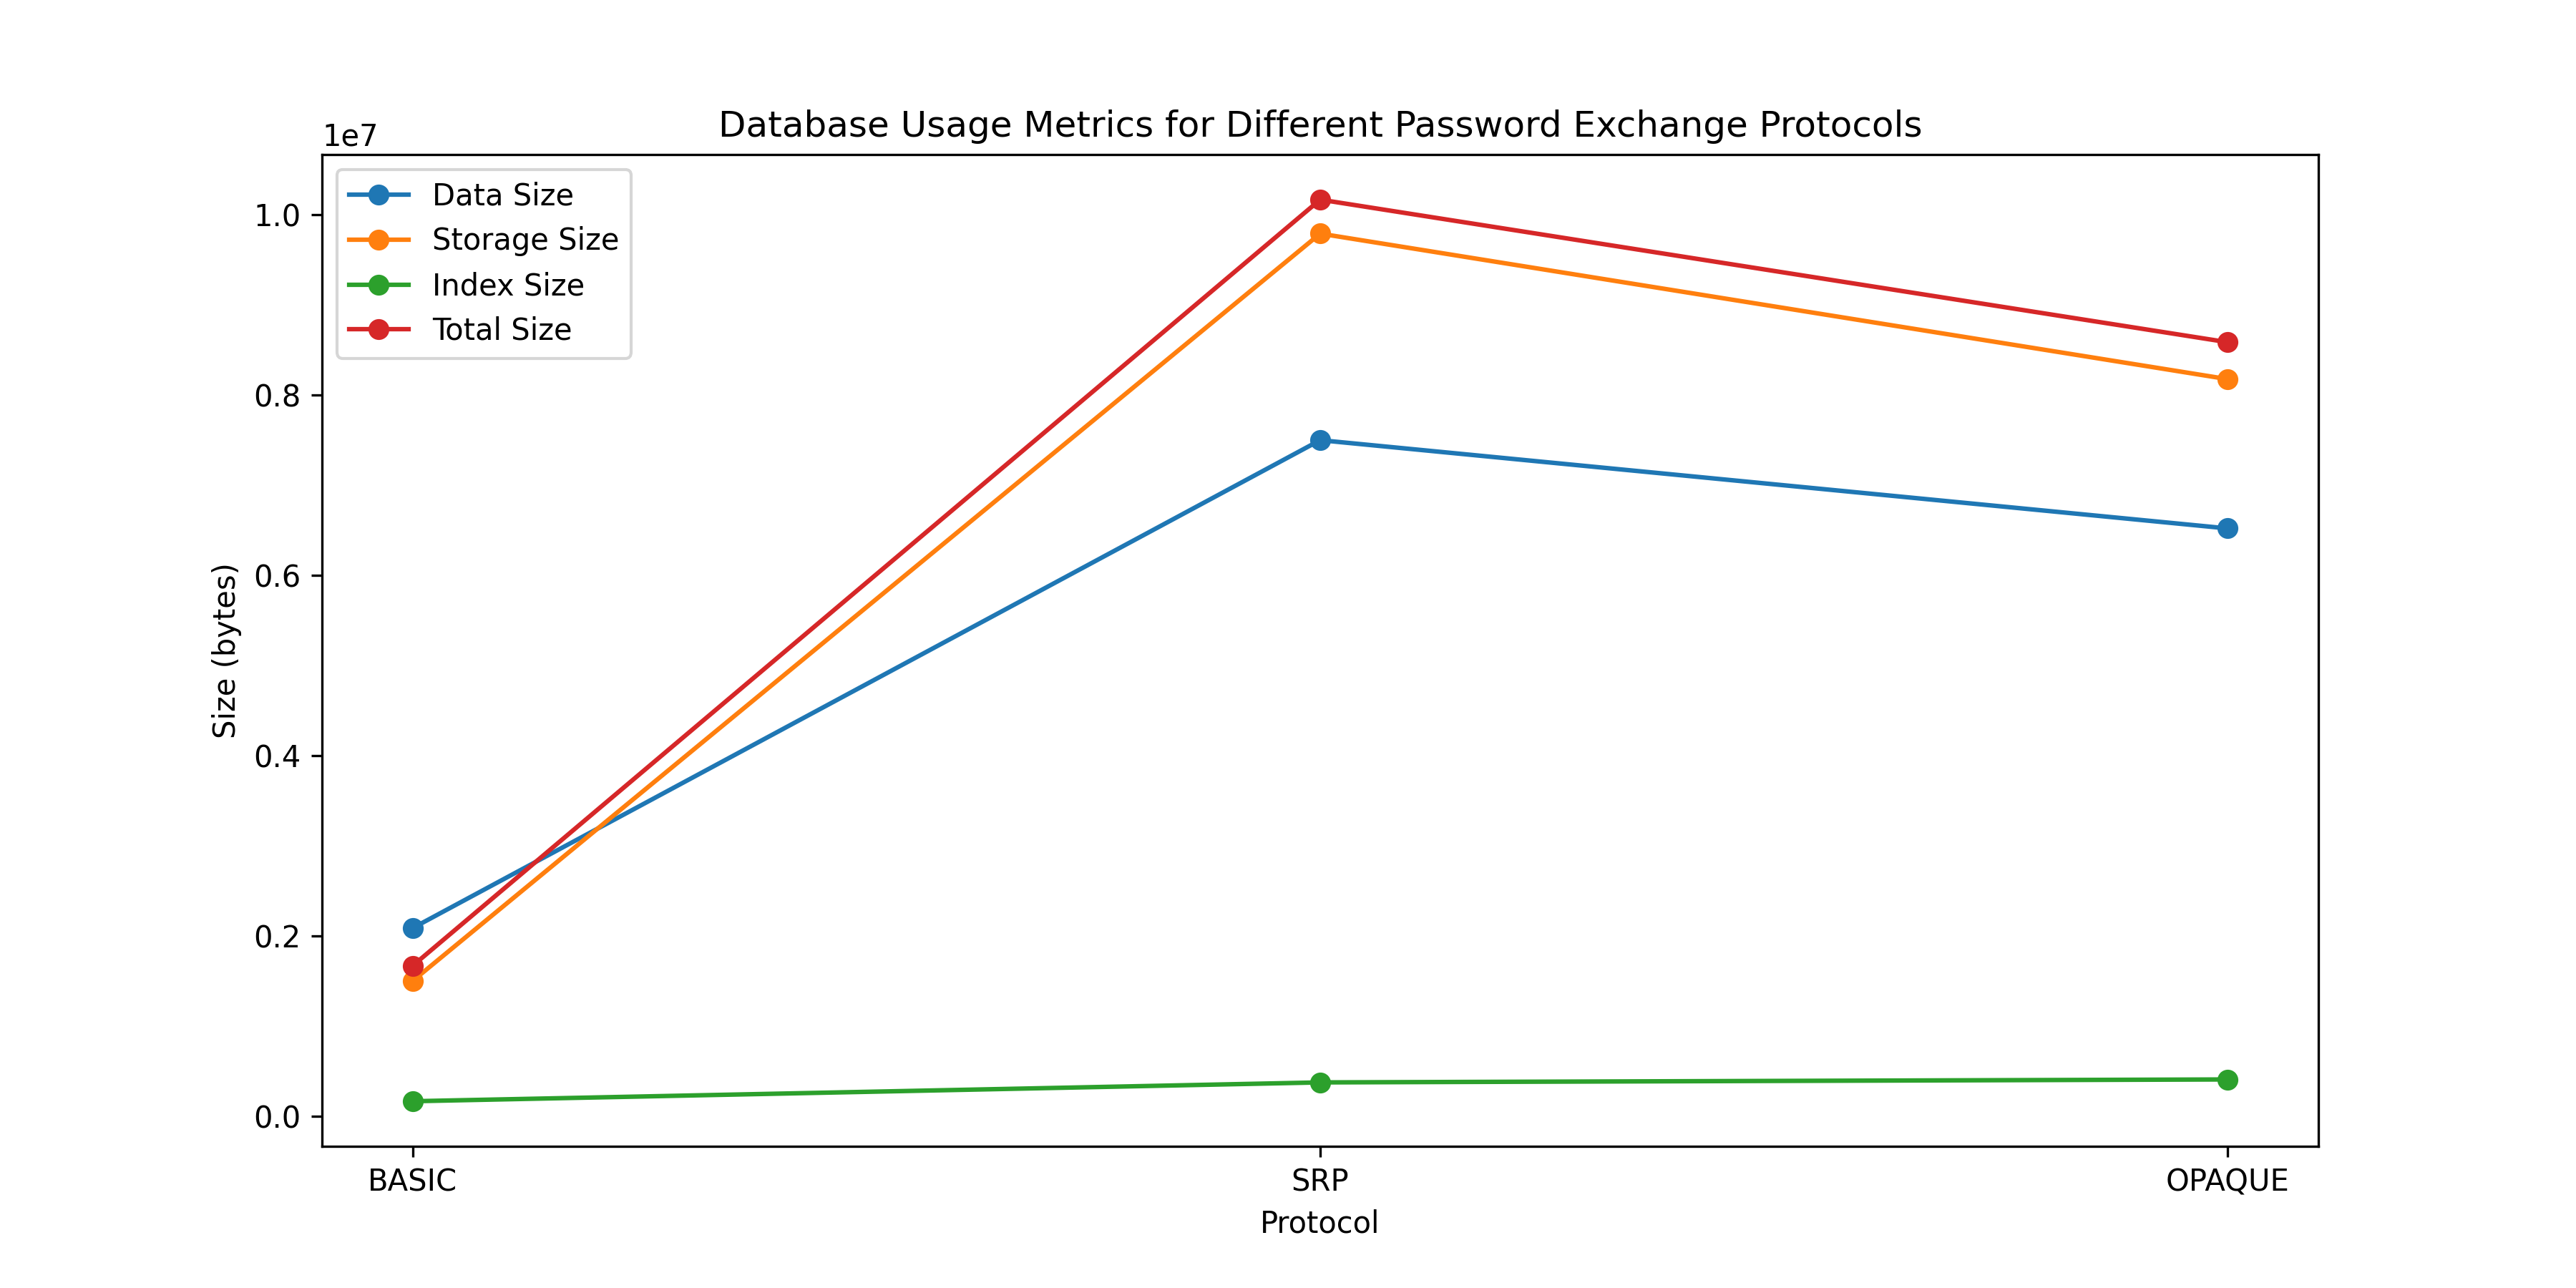
\includegraphics[width=0.4\textwidth]{./images/database_usage_metrics_line.png}
  \caption{Comparison of server-side storage usage}
  \label{fig:storage_usage}
\end{figure}

\subsection{Server-side Storage Usage}

Another aspect we investigated was the impact of the PAKE protocols on the server-side storage requirements. The storage usage is an important consideration, as PAKE protocols often require storing additional data, such as salts, session information, or encrypted client keys, to facilitate the authentication process.

From Figure \ref{fig:storage_usage}, our experiments revealed that the PAKE protocols, in general, required more storage space compared to the basic password-over-TLS authentication. The SRP protocol and the OPAQUE protocol had roughly the same storage usage, with the SRP protocol being slightly higher.

For the SRP protocol, the server needed to store the user's username, the generated secret value (V), and the salt (s) for each registered user, as evident from the figure. This additional data overhead amounted to an increase in storage requirements compared to the baseline password-over-TLS protocol.

The OPAQUE protocol, on the other hand, required storing a more complex data structure, including the encrypted envelope (E) containing the client's private key, the client's public key (CKp), and the salt (s) specific to each user's username. The storage usage for the OPAQUE protocol was slightly lower than the SRP protocol, but still significantly higher than the baseline, as can be observed in Figure \ref{fig:storage_usage}.

The Password Over TLS protocol, being the simplest in terms of server-side implementation, had the smallest storage footprint, as it only required storing the user's hashed password along with the salt. The storage usage for the Password Over TLS protocol was roughly half of the SRP and OPAQUE protocols, as depicted in the figure.

\begin{figure}[ht]
  \centering
  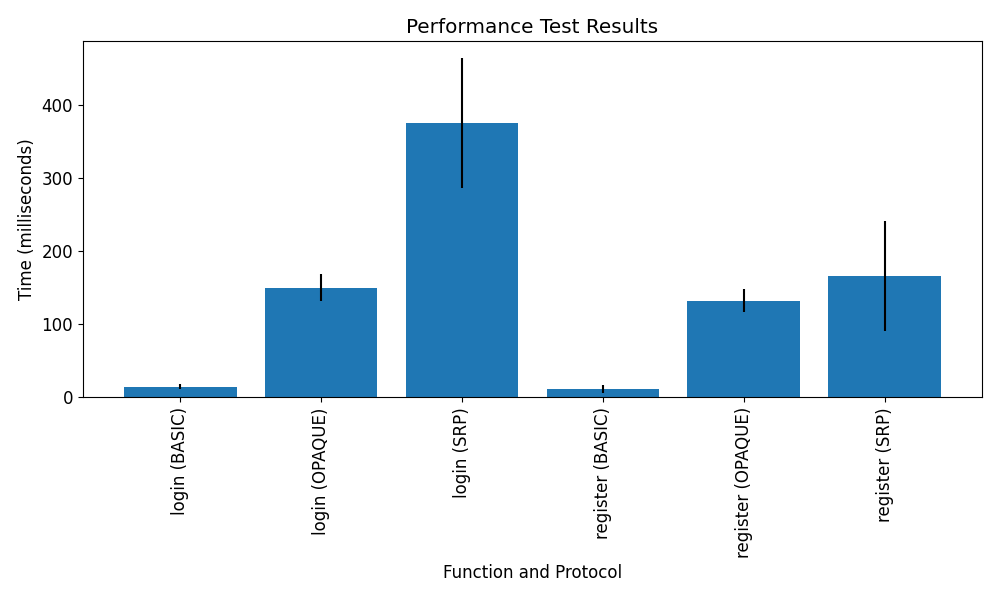
\includegraphics[width=0.4\textwidth]{./images/performance_test.png}
  \caption{Comparison of client-side per-request response times}
  \label{fig:performance_test}
\end{figure}

\subsection{Client-side experience}

In addition to the server-side performance metrics, we also examined the client-side experience during the authentication process. This was an important aspect to consider, as the user-perceived responsiveness and efficiency of the authentication flow can significantly impact the overall user experience.

The performance test results, as depicted in Figure \ref{fig:performance_test}, showed that the Password Over TLS (baseline) exhibited the fastest and most consistent response times throughout the simulation. The client-side request processing was relatively straightforward, involving the transmission of the username and password, followed by the server's verification and response. This simplicity translated to a smooth and responsive user experience, with minimal latency.

In contrast, the SRP protocol demonstrated significantly longer and more variable response times when compared to the Password Over TLS protocol, as evidenced by the figure. The client-side implementation of SRP required a more complex series of message exchanges, including the generation of ephemeral keys, the computation of the session proof, and the verification of the server's response. This additional computational overhead and the back-and-forth communication between the client and server resulted in a less responsive user experience, with some requests taking considerably longer to complete.

The OPAQUE protocol also exhibited longer response times compared to the Password Over TLS protocol, but the overall performance was better than the SRP protocol, as can be observed in the figure. The client-side operations in OPAQUE, such as the oblivious pseudorandom function (OPRF) and the encryption/decryption of the client's private key, were more optimized than the SRP protocol, leading to a more consistent and responsive user experience. However, the response times for OPAQUE were still noticeably longer than the baseline Password Over TLS protocol.